\section{Misje autonomiczne}

\begin{frame}{Skanowanie obszaru i optymalizacja tras}
    Ratownik szukający zaginionej osoby nie steruje dronem ręcznie nad całym lasem. Zadaje mu misję skanowania obszaru.
    \vspace{0.2cm}
    Jak wyznaczyć optymalną trasę z punktu $A$ do punktu $B$, zahaczając o inne ważne punkty? Z pomocą przychodzi teoria grafów i Problem Komiwojażera (TSP - Traveling Salesperson Problem).
    
    \begin{center}
    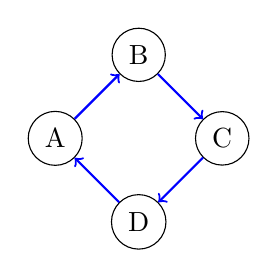
\begin{tikzpicture}[node distance=1.5cm, every node/.style={circle, draw, minimum size=0.5cm}]
        \node (1) at (0,0) {A};
        \node (2) [above right of=1] {B};
        \node (3) [below right of=2] {C};
        \node (4) [below right of=1] {D};
        
        \path[->, thick, blue]
            (1) edge (2)
            (2) edge (3)
            (3) edge (4)
            (4) edge (1);
    \end{tikzpicture}
    \end{center}
\end{frame}

\begin{frame}{Zaawansowane misje ratunkowe 3D}
    W rzeczywistości teren rzadko bywa płaski. Drony muszą uwzględniać wysokość (3D). 
    \vspace{0.5cm}
    
    \textbf{Demonstracja wideo:} Skanowanie obszaru poligonu, przeszukiwanie objętości cylindra i pościg za celem ruchomym.
    
    \begin{center}
    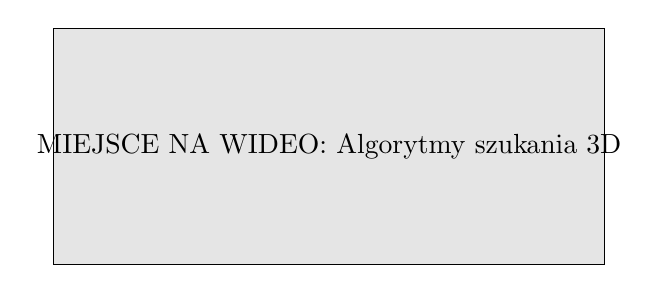
\begin{tikzpicture}
        \draw[fill=gray!20] (0,0) rectangle (7,3);
        \node at (3.5,1.5) {MIEJSCE NA WIDEO: Algorytmy szukania 3D};
    \end{tikzpicture}
    \end{center}
\end{frame}
